\documentclass[a4paper,twoside,12pt]{report}
% Richard Klein (2020,2021)

% Include Packages
%\usepackage[a4paper,inner=3.5cm,outer=2.5cm,top=2.5cm,bottom=2.5cm]{geometry}  % Set page margins
\usepackage{fullpage}
\usepackage{float}                  % Allows 'Here and Only Here' [H] for Floats
\usepackage{url}                    % \url{} command
\usepackage{charter}                  % Set font to Times
\usepackage{graphicx}               % \includegraphics
\usepackage{subfigure}              % Allow subfigures
\usepackage{amsmath}
\usepackage{amssymb}
\usepackage{amsthm}
\usepackage{booktabs}
\usepackage{parskip}
\usepackage[all]{nowidow}
\setnoclub[2]
\setnowidow[2]

\usepackage{csvsimple}
\usepackage{longtable}
\usepackage{listings}

% Referencing
% Provides \Vref and \vref to indicate where a reference is.
\usepackage{varioref} 
% Hyperlinks references
\usepackage[bookmarks=true,bookmarksopen=true]{hyperref} 
% Provides \Cref, \cref, \Vref, \vref to include the type of reference: fig/eqn/tbl
\usepackage{cleveref} 
% Setup Hyperref
\hypersetup{
  colorlinks   = true,              %Colours links instead of ugly boxes
  urlcolor     = blue,              %Colour for external hyperlinks
  linkcolor    = blue,              %Colour of internal links
  citecolor    = blue                %Colour of citations
}
% Names for Clever Ref
\crefname{table}{table}{tables}
\Crefname{table}{Table}{Tables}
\crefname{figure}{figure}{figures}
\Crefname{figure}{Figure}{Figures}
\crefname{equation}{equation}{equations}
\Crefname{equation}{Equation}{Equations}

% Wits Citation Style
\usepackage{natbib} % Force natbib.sty to put citation labels in the reference list
\makeatletter
\renewcommand\NAT@biblabel[1]{\def\citeauthoryear##1##2{##1 ##2}[#1]\hfill}
\renewcommand\NAT@bibsetup[1]{%
  \setlength{\itemsep}{\bibsep}\setlength{\parsep}{\z@}}
\def\@lbibitem[#1]#2{%
  \if\relax\@extra@b@citeb\relax\else
    \@ifundefined{br@#2\@extra@b@citeb}{}{%
     \@namedef{br@#2}{\@nameuse{br@#2\@extra@b@citeb}}}\fi
   \@ifundefined{b@#2\@extra@b@citeb}{\def\NAT@num{}}{\NAT@parse{#2}}%
   \item[\hfil\hyper@natanchorstart{#2\@extra@b@citeb}\@biblabel{#1}%
    \hyper@natanchorend]%
    \NAT@ifcmd#1(@)(@)\@nil{#2}}
\makeatother


\bibliographystyle{named-wits}
\bibpunct{[}{]}{;}{a}{}{}  % to get correct punctuation for bibliography
\setlength{\skip\footins}{1.5cm}
\newcommand{\citets}[1]{\citeauthor{#1}'s \citeyearpar{#1}}
\renewcommand\bibname{References}  

\pagestyle{headings}

\pagestyle{plain}
\pagenumbering{roman}

\renewenvironment{abstract}{\ \vfill\begin{center}\textbf{Abstract}\end{center}\addcontentsline{toc}{section}{Abstract}}{\vfill\vfill\newpage}
\newenvironment{declaration}{\ \vfill\begin{center}\textbf{Declaration}\end{center}\addcontentsline{toc}{section}{Declaration}}{\vfill\vfill\newpage}
\newenvironment{acknowledgements}{\ \vfill\begin{center}\textbf{Acknowledgements}\end{center}\addcontentsline{toc}{section}{Acknowledgements}}{\vfill\vfill\newpage}

\begin{document}
\onecolumn
\thispagestyle{empty}

\setcounter{page}{0}
\addcontentsline{toc}{chapter}{Preface}
\ 
\begin{center}
  \vfill
  {
  \huge \bf \textsc{Binary Search Trees and Order-Statistic Trees}\\
%  \large Subtitle\\[20pt]
  \large School of Computer Science \& Applied Mathematics\\
  \large University of the Witwatersrand\\[20pt]
  \normalsize
  Musawenkosi Gumpu\\
  2326254\\[20pt]
  \date{3 October 2023}
  }

  \vfill
  \vfill
  
\includegraphics[width=1.5cm]{images/wits}
  \vspace{10pt}\\
%  \small{Ethics Clearance Number: XX/XX/XX}\\[10pt]
  \small{A Comparative Analysis of Insertion and Deletion Methods in Binary Search Trees (BSTs)}\\
\end{center}
\vfill
\newpage

\pagestyle{plain}
\setcounter{page}{1}

% C++ Code formatting
\lstdefinestyle{mystyle}{
	language=C++,
	basicstyle=\ttfamily,
	keywordstyle=\color{blue},
	commentstyle=\color{green},
	numbers=left,
	numberstyle=\tiny\color{black},
	stepnumber=1,
	numbersep=5pt,
	frame=single,
	breaklines=true,
}

\phantomsection

%\begin{declaration}
%I, Musawenkosi Gumpu, hereby declare the contents of this research proposal to be my own work.
%This proposal is submitted for the degree of Bachelor of Science with Honours in Computer Science at the University of the %Witwatersrand.
%This work has not been submitted to any other university, or for any other degree.
%\end{declaration}

%\phantomsection
%\begin{acknowledgements}
%Special thanks to my supervisors - Dr Steven James and Prof. Benjamin Rosman - for their help in discovering a potential %alternative approach to developing a model capable of generating content.
%\end{acknowledgements}


\phantomsection
\addcontentsline{toc}{section}{Table of Contents}
\tableofcontents
\newpage
\phantomsection
\addcontentsline{toc}{section}{List of Figures}

\listoffigures

\begin{figure}[h]
	\centering
	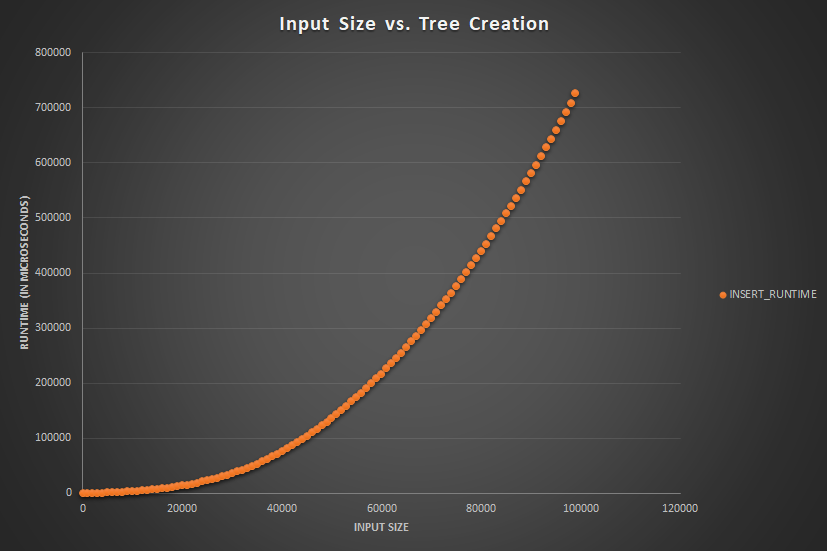
\includegraphics[width=1.0\textwidth]{images/size-vs-build-time}
	\caption{Comparison of input size and expected build time.}
	\label{fig:size-vs-runtime}
\end{figure}
\begin{figure}[h]
	\centering
	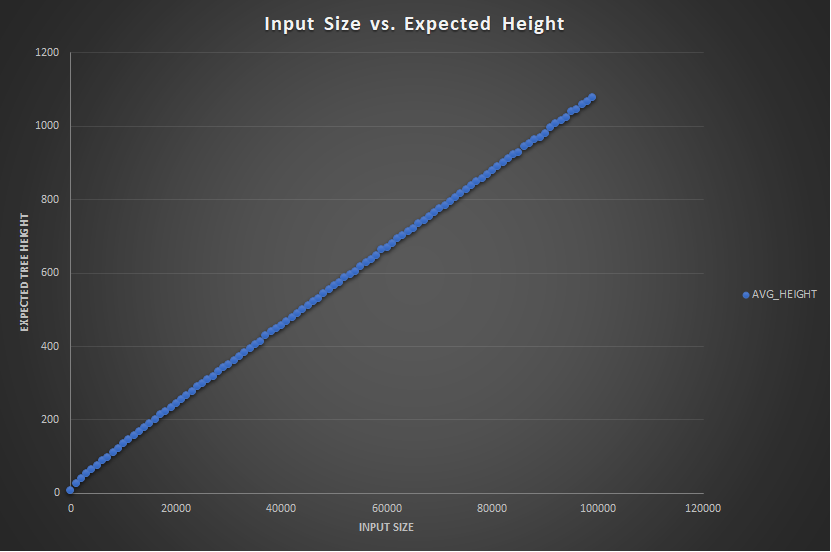
\includegraphics[width=1.0\textwidth]{images/size-vs-tree-height}
	\caption{Comparison of input size and expected tree height.}
	\label{fig:size-vs-tree-height}
\end{figure}
\begin{figure}[h]
	\centering
	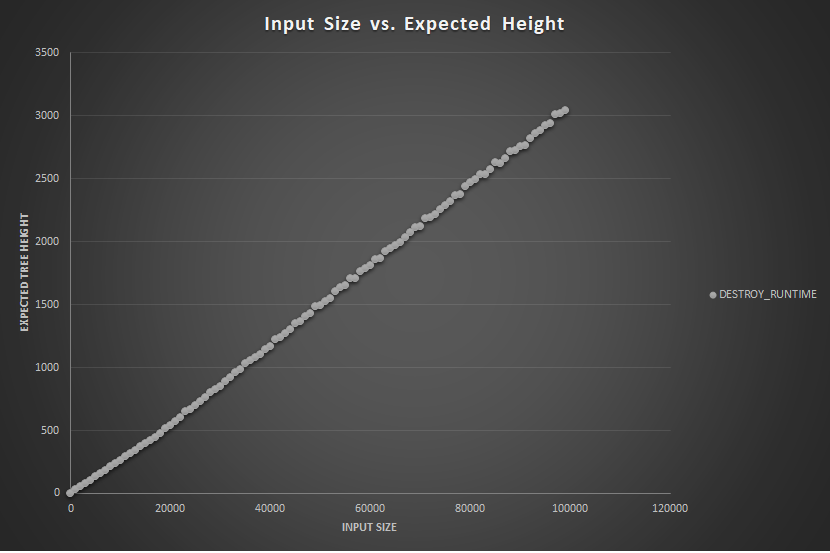
\includegraphics[width=1.0\textwidth]{images/size-vs-destroy-time}
	\caption{Comparison of input size and expected destroy time.}
	\label{fig:size-vs-destroy-time}
\end{figure}

\newpage
\phantomsection

\newpage
\pagenumbering{arabic}

\chapter{Introduction}
In this study, we aim to conduct a comprehensive analysis of Binary Search Trees (BSTs) by comparing the average insertion time when populating a BST with an array of randomly shuffled elements across varying input sizes. Additionally, we seek to experimentally validate the expected height of insertions in BSTs, that it is indeed of $O(\log n)$ complexity. Furthermore, we will assess the average time required for the destruction of BSTs.
We also aim to determine a means to create an augmented BST which closely resembles that of a Order Statistic Tree that is not a Red-Black Tree, but has the size property used to determine the rank of a node in the tree.

We also explore augmented BSTs that follow the structure of an Order Statistic Tree, without being limited to the constraints of Red-Black Trees. This augmented BST will maintain a size property that allows us to efficiently determine the rank of a node within the tree.



\chapter{Objective}
The primary objective of this experiment is to empirically demonstrate that a randomly constructed Binary Search Tree (BST) using $n$ distinct keys exhibits an expected height of $O(\log n)$. By conducting a series of experiments and data analysis, we aim to confirm that the growth in height of a BST is logarithmic in nature to the input size $n$. This is useful to support the fundamental property BSTs, enabling us to better understand the practical application of the implemented insertion and destruction methods.

We also aim to develop an augmented BST that resembles the functionality of an Order Statistic Tree while avoiding the constraints of Red-Black Trees. This augmented BST will have each node incorporate a size property, will allow us to efficiently determine the rank of a node within the tree.

\chapter{Methodology}
\section{Experimental Setup}
The experimental implementations were coded in C++. The results obtained from the experiment were recorded in a comma-separated values (CSV) file.
\subsection{Range of Dimensions \& Key Values}
To investigate the performance of BSTs, we populate them with randomly shuffled arrays of varying input sizes. Our input sizes range from $16$ to $100,000$ elements, with keys represented as random integers falling within the range $[1, 100]$. This comprehensive range of inputs allows us to conduct an empirical analysis and compare our experimental findings with theoretical expectations. Specifically, we aim to verify that the average insertion time exhibits linearithmic behaviour, denoted as $O(n \log n)$, as each key insertion taking $\Theta(n)$ operations, may each take up to $O(\log n)$ time.

\subsection{Number of Trees}
To ensure the robustness and reliability of our results, we conducted 30 iterations for each input size, making use of different sets of random key values. This allowed us to accurately observe the performance of BST creation, destruction, and expected height analysis across various scenarios, aligning our conclusions with the theoretical basis of what was stated.

\chapter{Analysis of BST}
It is essential to note that a standard Binary Search Tree (BST) can become unbalanced, leading to the worst-case scenario where a subtree resembles a linked list. In such situations, certain operations may have a time complexity of $O(n)$ instead of the expected $O(\log n)$ that we aim to observe.

In the following sections, we present the outcomes of our experiments (see Table \ref{tab:results}) and discuss the implications of our findings.

\section{Expected Height}
Our analysis of the expected height of a BST aligns with the behavior of a logarithmic function, as demonstrated in Figure \ref{fig:size-vs-tree-height}.

\subsection{Average Insertion Runtime}
The graph representing the average insertion runtime (Figure \ref{fig:size-vs-runtime}) exhibits a behaviour that appears similar to that of a quadratic function, $O(n^2)$. This observation can be justified by the fact that random shuffling does not guarantee balanced tree formations during each key insertion, which inherently takes $O(n)$ time. Consequently, in the worst-case scenario, the insertion process may indeed exhibit a time complexity resembling that of a linked list, which is $O(n)$.

\subsection{Tree Destruction Runtime}
To efficiently destroy the BST, we decided to perform a sequential deletion of the root node of the tree. This can be motivated by the inefficiency of using the randomly shuffled array for tree destruction, as it would require searching for the keys, a task that can take $O(n)$ time in the worst-case scenario of a highly unbalanced tree with $n$ nodes. Additionally, the deletion of a node can have a time complexity of up to $O(h)$, where $h$ denotes the height of the tree. This is due to the possibility of needing to find a successor node in cases where the node being deleted has two children. 
One can observe this linear trend from (Figure \ref{fig:size-vs-destroy-time}). Making use of the randomly shuffled array as a reference to delete the tree would bring in the additional cost of having to search for the node to be deleted, possibly making the tree destruction runtime reach $O(n^2)$. This justifies the approach of sequentially deleting the root node of the tree.


\chapter{Improvement to BST: The Size Attribute}
Augmenting a Binary Search Tree (BST) by introducing the "size" attribute to each node allows us to determine the rank of a node within the tree and efficiently locate the i-th order statistic node, making BSTs even more versatile.

In initializing a node, it has an initial size of 0. Since we are not implementing Red-Black Tree constraints, a check is performed to determine if a node has any children before obtaining its size property. This check ensures that the size attribute remains accurate as we manipulate the tree's structure, preventing errors relating to a null pointer reference.

The size of a node, denoted as $x$, is calculated using the following formula:

$size(x)=size(leftChild)+size(rightChild)+1$

\section{Maintaining Node Sizes on Key Insertion}
To maintain the sizes of all nodes after inserting a new key, we iteratively update the sizes of the nodes along the path to the root node with (\ref{insertUpdate}). We use the same code for key insertion as shown in \ref{app:tree-insert}. It is after inserting the key that it is necessary to update the sizes of the nodes from its inserted position to the root position. (\ref{insertUpdate}) guarantees that after insertion, the sizes of all nodes are correct, in being the updated size of the respective subtree.

\newpage
\subsection{Size Update of Inserted Node After Insert} \label{insertUpdate}
\begin{lstlisting}[style=mystyle]
void insertupdate(OS_Node *currNode) {
	while (currNode != nullptr) {
		currNode.size = (currNode.left == nullptr ? 0 : currNode.left.size) + (currNode.right == nullptr ? 0 : currNode.right.size) + 1;
		currNode = currNode.parent;
	}
}
\end{lstlisting}

\section{Maintaining Node Sizes on Key Deletion}

When performing key deletion using the same code as $TREE-DELETE$ in \ref{app:tree-delete}, there are two fundamental cases to consider, each requiring specific adjustments to maintain the accuracy of the size attributes.

1. \textbf{Deletion with One Child:}

In the first case, when the node being deleted has only one child, the only child becomes the next successor. To ensure that the sizes of ancestors of the node to be deleted are correctly updated, we decrement their sizes by 1.

2. \textbf{Deletion with Two Children:}

In the second case, when the node being deleted has two children, the sizes of ancestors of the chosen successor - given by the minimum node of the left child's subtree - need to be decremented by 1. 

We perform the \ref{deleteUpdate} operation before executing the transplant operation. This simplifies the process of not needing to perform any complex calculations on which node sizes need to be updated. We also maintain the integrity of the size attributes, ensuring that after key deletion, the accuracy in the sizes of the nodes is still maintained.

\subsection{Size Update of Deleted node Before Deletion} \label{deleteUpdate}
\begin{lstlisting}[style=mystyle] 
void deleteUpdateSize(OS_Node *currNode) {
	while (currNode != nullptr) {
		currNode.size -= 1;
		currNode = currNode.parent;
	}
}
\end{lstlisting}


\chapter{Conclusion}
In conclusion, the Binary Search Tree (BST) and its augmented version, which includes the size property, have produced the following results.

When randomly constructing the BST, its expected height has consistently remained close to an average of $O(\log n)$. This ensures that efficient search operations are possible without incurring excessive overhead in setting up the data structure.

Insertion, although not strictly linearithmic and exhibiting a quadratic trend, can be improved by incorporating the AVL property or adopting the Red-Black constraints. However, this improvement comes at the cost of a more complex implementation.

Destroying the tree by iteratively deleting the root node results in a linear trend, as observed. This approach was well-justified when compared to using each key in the randomly shuffled list used to construct the tree.

Including the size property in nodes is a simple implementation that enables the ability to determine the rank of a node and retrieve order statistic nodes. Maintaining this property is fairly straightforward and opens up opportunities for various applications that can contribute significantly to solving complex computational challenges.


\appendix
\chapter{Appendix}\label{app:extra}


\section{TREE-INSERT}\label{app:tree-insert}
As adapted to C++ from the algorithm provided by \citet{Cormen2009}
\begin{lstlisting}[style=mystyle]
void TREE-INSERT(BST& T, Node* z) {
	y = nullptr;
	x = T.root;
	while (x != nullptr)
		y = x;
		if (z.key < x.key)
			x = x.left;
		else 
			x = x.right;
	z.p = y;
	if (y == nullptr)
		T.root = z;
	else if (z.key < y.key)
		y.left = z;
	else 
		y.right = z;
		
	\\ For maintaining OS_BST sizes, insertUpdate(z) is called
}
\end{lstlisting}

\newpage
\section{TREE-DELETE}\label{app:tree-delete}
As adapted to C++ from the algorithm provided by \citet{Cormen2009}
\begin{lstlisting}[style=mystyle]
void TREE-DELETE(BST& T, Node* z) {
	if (z.left == nullptr) {
		\\ For maintaining OS_BST node sizes, deleteUpdateSize(z) is called here
		TRANSPLANT(T, z, z.right);
	}
	else if (z.right == nullptr) {
		\\ For maintaining OS_BST node sizes, deleteUpdateSize(z) is called here
		TRANSPLANT(T, z, z.left);
	}
	else {
		y = TREE-MINIMUM(z.right);
		
		\\ For maintaining OS_BST node sizes, deleteUpdateSize(y) is called here
		
		if (y.p != z) {
			TRANSPLANT(T, y, y.right);
			y.right = z.right;
			y.right.p = y;
		}
		TRANSPLANT(T, z, y);
		y.left = z.left;
		y.left.p = y;
	}
	
}
\end{lstlisting}

\addcontentsline{toc}{section}{Tabular Results}
\listoftables
\section{Tabular Results}\label{tab:results}

	\begin{longtable}{|l|l|l|l|}
		\hline
		SIZE  & AVG\_HEIGHT & INSERT\_RUNTIME & DESTROY\_RUNTIME \\ \hline
		16    & 7           & 2               & 0                \\ \hline
		144   & 14          & 50              & 14               \\ \hline
		272   & 18          & 80              & 23               \\ \hline
		400   & 20          & 112             & 33               \\ \hline
		528   & 21          & 156             & 40               \\ \hline
		656   & 23          & 143             & 39               \\ \hline
		784   & 26          & 154             & 45               \\ \hline
		912   & 27          & 180             & 56               \\ \hline
		1040  & 30          & 189             & 58               \\ \hline
		1168  & 30          & 236             & 73               \\ \hline
		1296  & 32          & 287             & 86               \\ \hline
		1424  & 34          & 316             & 90               \\ \hline
		1552  & 35          & 331             & 93               \\ \hline
		1680  & 37          & 342             & 101              \\ \hline
		1808  & 39          & 418             & 120              \\ \hline
		1936  & 40          & 434             & 122              \\ \hline
		2064  & 41          & 501             & 149              \\ \hline
		2192  & 44          & 491             & 132              \\ \hline
		2320  & 46          & 528             & 143              \\ \hline
		2448  & 47          & 606             & 158              \\ \hline
		2576  & 48          & 599             & 155              \\ \hline
		2704  & 51          & 614             & 155              \\ \hline
		2832  & 51          & 649             & 166              \\ \hline
		2960  & 53          & 712             & 183              \\ \hline
		3088  & 54          & 745             & 179              \\ \hline
		3216  & 56          & 783             & 187              \\ \hline
		3344  & 57          & 837             & 190              \\ \hline
		3472  & 60          & 974             & 220              \\ \hline
		3600  & 62          & 903             & 204              \\ \hline
		3728  & 62          & 988             & 224              \\ \hline
		3856  & 64          & 1015            & 220              \\ \hline
		3984  & 66          & 1084            & 230              \\ \hline
		4112  & 67          & 1128            & 238              \\ \hline
		4240  & 68          & 1188            & 239              \\ \hline
		4368  & 70          & 1246            & 245              \\ \hline
		4496  & 71          & 1298            & 247              \\ \hline
		4624  & 74          & 1363            & 260              \\ \hline
		4752  & 74          & 1424            & 266              \\ \hline
		4880  & 75          & 1479            & 270              \\ \hline
		5008  & 77          & 1584            & 277              \\ \hline
		5136  & 79          & 1627            & 279              \\ \hline
		5264  & 80          & 1799            & 310              \\ \hline
		5392  & 82          & 1773            & 304              \\ \hline
		5520  & 83          & 1865            & 305              \\ \hline
		5648  & 85          & 1950            & 313              \\ \hline
		5776  & 85          & 2032            & 320              \\ \hline
		5904  & 87          & 2142            & 344              \\ \hline
		6032  & 90          & 2232            & 358              \\ \hline
		6160  & 91          & 2323            & 364              \\ \hline
		6288  & 93          & 2432            & 365              \\ \hline
		6416  & 94          & 2505            & 366              \\ \hline
		6544  & 95          & 2583            & 378              \\ \hline
		6672  & 96          & 2702            & 388              \\ \hline
		6800  & 98          & 2792            & 390              \\ \hline
		6928  & 100         & 2940            & 405              \\ \hline
		7056  & 100         & 2957            & 395              \\ \hline
		7184  & 103         & 3210            & 442              \\ \hline
		7312  & 104         & 3310            & 429              \\ \hline
		7440  & 105         & 3332            & 422              \\ \hline
		7568  & 107         & 3379            & 430              \\ \hline
		7696  & 107         & 3520            & 431              \\ \hline
		7824  & 110         & 3694            & 452              \\ \hline
		7952  & 111         & 4237            & 487              \\ \hline
		8080  & 113         & 4171            & 495              \\ \hline
		8208  & 114         & 4340            & 507              \\ \hline
		8336  & 117         & 4559            & 519              \\ \hline
		8464  & 117         & 4507            & 500              \\ \hline
		8592  & 118         & 4709            & 529              \\ \hline
		8720  & 121         & 4612            & 494              \\ \hline
		8848  & 119         & 4759            & 503              \\ \hline
		8976  & 123         & 5095            & 523              \\ \hline
		9104  & 125         & 5037            & 532              \\ \hline
		9232  & 126         & 5289            & 522              \\ \hline
		9360  & 127         & 5641            & 550              \\ \hline
		9488  & 129         & 5453            & 515              \\ \hline
		9616  & 130         & 5548            & 521              \\ \hline
		9744  & 131         & 5683            & 526              \\ \hline
		9872  & 134         & 5835            & 540              \\ \hline
		10000 & 135         & 15555           & 1333             \\ \hline
		10128 & 135         & 19721           & 1710             \\ \hline
		10256 & 137         & 20326           & 1703             \\ \hline
		10384 & 139         & 21444           & 1735             \\ \hline
		10512 & 140         & 21903           & 1802             \\ \hline
		10640 & 142         & 22126           & 1775             \\ \hline
		10768 & 141         & 28920           & 2427             \\ \hline
		10896 & 146         & 27215           & 2212             \\ \hline
		11024 & 144         & 27440           & 2281             \\ \hline
		11152 & 148         & 26593           & 2024             \\ \hline
		11280 & 149         & 26091           & 1918             \\ \hline
		11408 & 149         & 26555           & 1944             \\ \hline
		11536 & 152         & 12505           & 916              \\ \hline
		11664 & 154         & 7232            & 531              \\ \hline
		11792 & 154         & 7305            & 532              \\ \hline
		11920 & 156         & 8532            & 625              \\ \hline
		12048 & 157         & 7812            & 562              \\ \hline
		12176 & 159         & 8001            & 554              \\ \hline
		12304 & 160         & 8122            & 561              \\ \hline
		12432 & 162         & 8471            & 594              \\ \hline
		12560 & 164         & 8946            & 593              \\ \hline
		12688 & 164         & 9062            & 601              \\ \hline
		12816 & 166         & 9399            & 619              \\ \hline
		12944 & 168         & 10033           & 630              \\ \hline
		13072 & 168         & 10323           & 677              \\ \hline
		13200 & 170         & 10377           & 665              \\ \hline
		13328 & 172         & 10388           & 629              \\ \hline
		13456 & 172         & 10543           & 653              \\ \hline
		13584 & 175         & 11159           & 674              \\ \hline
		13712 & 176         & 10898           & 665              \\ \hline
		13840 & 178         & 11533           & 686              \\ \hline
		13968 & 179         & 11902           & 703              \\ \hline
		14096 & 179         & 13366           & 780              \\ \hline
		14224 & 182         & 14475           & 921              \\ \hline
		14352 & 182         & 14613           & 824              \\ \hline
		14480 & 187         & 13117           & 728              \\ \hline
		14608 & 185         & 12837           & 706              \\ \hline
		14736 & 187         & 13145           & 722              \\ \hline
		14864 & 189         & 13338           & 723              \\ \hline
		14992 & 191         & 13707           & 735              \\ \hline
		15120 & 191         & 14090           & 744              \\ \hline
		15248 & 193         & 14330           & 736              \\ \hline
		15376 & 195         & 14580           & 774              \\ \hline
		15504 & 194         & 14884           & 788              \\ \hline
		15632 & 198         & 14990           & 748              \\ \hline
		15760 & 198         & 14920           & 731              \\ \hline
		15888 & 199         & 15417           & 796              \\ \hline
		16016 & 201         & 15785           & 771              \\ \hline
		16144 & 202         & 16432           & 809              \\ \hline
		16272 & 203         & 16430           & 822              \\ \hline
		16400 & 207         & 16453           & 788              \\ \hline
		16528 & 206         & 16778           & 791              \\ \hline
		16656 & 209         & 17066           & 788              \\ \hline
		16784 & 211         & 17510           & 810              \\ \hline
		16912 & 210         & 17546           & 829              \\ \hline
		17040 & 214         & 18521           & 839              \\ \hline
		17168 & 214         & 18140           & 827              \\ \hline
		17296 & 216         & 18578           & 842              \\ \hline
		17424 & 215         & 19774           & 1033             \\ \hline
		17552 & 219         & 19173           & 891              \\ \hline
		17680 & 221         & 18498           & 820              \\ \hline
		17808 & 220         & 18640           & 803              \\ \hline
		17936 & 222         & 19086           & 828              \\ \hline
		18064 & 225         & 19112           & 807              \\ \hline
		18192 & 226         & 19484           & 850              \\ \hline
		18320 & 228         & 20091           & 830              \\ \hline
		18448 & 226         & 20090           & 841              \\ \hline
		18576 & 229         & 20364           & 864              \\ \hline
		18704 & 229         & 20349           & 819              \\ \hline
		18832 & 232         & 20719           & 844              \\ \hline
		18960 & 234         & 21170           & 850              \\ \hline
		19088 & 234         & 21718           & 867              \\ \hline
		19216 & 235         & 21987           & 882              \\ \hline
		19344 & 240         & 21889           & 860              \\ \hline
		19472 & 238         & 22288           & 862              \\ \hline
		19600 & 241         & 22637           & 900              \\ \hline
		19728 & 243         & 32033           & 1283             \\ \hline
		19856 & 244         & 23317           & 883              \\ \hline
		19984 & 245         & 23760           & 886              \\ \hline
		20112 & 246         & 23876           & 924              \\ \hline
		20240 & 249         & 24562           & 902              \\ \hline
		20368 & 248         & 25024           & 906              \\ \hline
		20496 & 247         & 24738           & 903              \\ \hline
		20624 & 251         & 25317           & 922              \\ \hline
		20752 & 252         & 25107           & 915              \\ \hline
		20880 & 254         & 25842           & 926              \\ \hline
		21008 & 256         & 26165           & 941              \\ \hline
		21136 & 256         & 26537           & 950              \\ \hline
		21264 & 257         & 27058           & 956              \\ \hline
		21392 & 259         & 27477           & 949              \\ \hline
		21520 & 261         & 27600           & 946              \\ \hline
		21648 & 264         & 28095           & 981              \\ \hline
		21776 & 266         & 28512           & 965              \\ \hline
		21904 & 267         & 28894           & 1004             \\ \hline
		22032 & 267         & 28921           & 981              \\ \hline
		22160 & 266         & 29418           & 982              \\ \hline
		22288 & 270         & 29539           & 999              \\ \hline
		22416 & 270         & 30680           & 1009             \\ \hline
		22544 & 273         & 30841           & 1014             \\ \hline
		22672 & 274         & 31017           & 1031             \\ \hline
		22800 & 274         & 31620           & 1033             \\ \hline
		22928 & 275         & 31708           & 1032             \\ \hline
		23056 & 277         & 32152           & 1025             \\ \hline
		23184 & 282         & 32139           & 1043             \\ \hline
		23312 & 280         & 33001           & 1042             \\ \hline
		23440 & 283         & 33191           & 1066             \\ \hline
		23568 & 283         & 33511           & 1073             \\ \hline
		23696 & 285         & 34287           & 1069             \\ \hline
		23824 & 288         & 34686           & 1071             \\ \hline
		23952 & 286         & 35005           & 1071             \\ \hline
		24080 & 289         & 35150           & 1100             \\ \hline
		24208 & 292         & 35450           & 1106             \\ \hline
		24336 & 291         & 36245           & 1138             \\ \hline
		24464 & 292         & 37570           & 1123             \\ \hline
		24592 & 294         & 39117           & 1135             \\ \hline
		24720 & 294         & 41226           & 1279             \\ \hline
		24848 & 296         & 41985           & 1199             \\ \hline
		24976 & 299         & 39894           & 1195             \\ \hline
		25104 & 302         & 40061           & 1167             \\ \hline
		25232 & 301         & 41547           & 1321             \\ \hline
		25360 & 302         & 42154           & 1240             \\ \hline
		25488 & 307         & 42277           & 1265             \\ \hline
		25616 & 305         & 42627           & 1274             \\ \hline
		25744 & 307         & 40939           & 1213             \\ \hline
		25872 & 306         & 42144           & 1185             \\ \hline
		26000 & 307         & 41825           & 1182             \\ \hline
		26128 & 310         & 42607           & 1193             \\ \hline
		26256 & 312         & 42931           & 1159             \\ \hline
		26384 & 314         & 43109           & 1195             \\ \hline
		26512 & 315         & 43304           & 1222             \\ \hline
		26640 & 318         & 44202           & 1205             \\ \hline
		26768 & 320         & 44213           & 1212             \\ \hline
		26896 & 319         & 45252           & 1258             \\ \hline
		27024 & 318         & 45790           & 1224             \\ \hline
		27152 & 319         & 46054           & 1228             \\ \hline
		27280 & 322         & 46462           & 1227             \\ \hline
		27408 & 325         & 46456           & 1220             \\ \hline
		27536 & 326         & 47685           & 1240             \\ \hline
		27664 & 328         & 48003           & 1250             \\ \hline
		27792 & 327         & 48399           & 1245             \\ \hline
		27920 & 329         & 48616           & 1263             \\ \hline
		28048 & 331         & 49424           & 1265             \\ \hline
		28176 & 332         & 49631           & 1258             \\ \hline
		28304 & 334         & 50688           & 1277             \\ \hline
		28432 & 333         & 50855           & 1299             \\ \hline
		28560 & 336         & 51407           & 1308             \\ \hline
		28688 & 341         & 52106           & 1310             \\ \hline
		28816 & 341         & 52148           & 1348             \\ \hline
		28944 & 343         & 53079           & 1295             \\ \hline
		29072 & 343         & 53377           & 1319             \\ \hline
		29200 & 342         & 53221           & 1349             \\ \hline
		29328 & 342         & 54454           & 1304             \\ \hline
		29456 & 347         & 53432           & 1322             \\ \hline
		29584 & 347         & 54980           & 1361             \\ \hline
		29712 & 348         & 55466           & 1333             \\ \hline
		29840 & 352         & 56230           & 1350             \\ \hline
		29968 & 352         & 56782           & 1374             \\ \hline
		30096 & 353         & 57268           & 1357             \\ \hline
		30224 & 355         & 57230           & 1412             \\ \hline
		30352 & 359         & 58241           & 1350             \\ \hline
		30480 & 359         & 58393           & 1380             \\ \hline
		30608 & 356         & 59115           & 1357             \\ \hline
		30736 & 361         & 59494           & 1375             \\ \hline
		30864 & 361         & 60355           & 1371             \\ \hline
		30992 & 363         & 61280           & 1392             \\ \hline
		31120 & 365         & 61789           & 1405             \\ \hline
		31248 & 366         & 61705           & 1443             \\ \hline
		31376 & 367         & 62942           & 1408             \\ \hline
		31504 & 369         & 62127           & 1419             \\ \hline
		31632 & 371         & 68727           & 1772             \\ \hline
		31760 & 373         & 68037           & 1615             \\ \hline
		31888 & 373         & 70395           & 1698             \\ \hline
		32016 & 375         & 71459           & 1654             \\ \hline
		32144 & 374         & 66226           & 1446             \\ \hline
		32272 & 377         & 65818           & 1459             \\ \hline
		32400 & 380         & 67579           & 1496             \\ \hline
		32528 & 379         & 66585           & 1438             \\ \hline
		32656 & 381         & 67927           & 1442             \\ \hline
		32784 & 382         & 68874           & 1486             \\ \hline
		32912 & 384         & 68784           & 1461             \\ \hline
		33040 & 386         & 69697           & 1513             \\ \hline
		33168 & 384         & 70599           & 1540             \\ \hline
		33296 & 384         & 71704           & 1514             \\ \hline
		33424 & 390         & 71272           & 1528             \\ \hline
		33552 & 389         & 72819           & 1614             \\ \hline
		33680 & 390         & 72835           & 1508             \\ \hline
		33808 & 392         & 72392           & 1516             \\ \hline
		33936 & 394         & 71935           & 1521             \\ \hline
		34064 & 396         & 74547           & 1533             \\ \hline
		34192 & 400         & 75049           & 1593             \\ \hline
		34320 & 401         & 76458           & 1559             \\ \hline
		34448 & 399         & 76388           & 1554             \\ \hline
		34576 & 402         & 76893           & 1606             \\ \hline
		34704 & 405         & 78037           & 1612             \\ \hline
		34832 & 408         & 78959           & 1566             \\ \hline
		34960 & 406         & 79302           & 1567             \\ \hline
		35088 & 405         & 79818           & 1560             \\ \hline
		35216 & 408         & 78921           & 1573             \\ \hline
		35344 & 409         & 80307           & 1593             \\ \hline
		35472 & 414         & 80540           & 1592             \\ \hline
		35600 & 414         & 80646           & 1632             \\ \hline
		35728 & 411         & 81866           & 1615             \\ \hline
		35856 & 417         & 83284           & 1624             \\ \hline
		35984 & 416         & 84341           & 1631             \\ \hline
		36112 & 419         & 83663           & 1610             \\ \hline
		36240 & 418         & 84823           & 1646             \\ \hline
		36368 & 422         & 84502           & 1623             \\ \hline
		36496 & 423         & 85052           & 1634             \\ \hline
		36624 & 423         & 87290           & 1663             \\ \hline
		36752 & 424         & 86924           & 1672             \\ \hline
		36880 & 426         & 87211           & 1696             \\ \hline
		37008 & 426         & 88872           & 1679             \\ \hline
		37136 & 427         & 90042           & 1680             \\ \hline
		37264 & 430         & 89930           & 1711             \\ \hline
		37392 & 431         & 90124           & 1712             \\ \hline
		37520 & 432         & 90757           & 1726             \\ \hline
		37648 & 434         & 92253           & 1870             \\ \hline
		37776 & 439         & 93179           & 1732             \\ \hline
		37904 & 438         & 93773           & 1754             \\ \hline
		38032 & 441         & 95026           & 1746             \\ \hline
		38160 & 439         & 93265           & 1739             \\ \hline
		38288 & 445         & 94072           & 1697             \\ \hline
		38416 & 440         & 97807           & 1785             \\ \hline
		38544 & 446         & 95913           & 1769             \\ \hline
		38672 & 446         & 96909           & 1741             \\ \hline
		38800 & 445         & 97483           & 1773             \\ \hline
		38928 & 448         & 97918           & 1757             \\ \hline
		39056 & 447         & 98276           & 1781             \\ \hline
		39184 & 450         & 100113          & 1817             \\ \hline
		39312 & 451         & 100917          & 1772             \\ \hline
		39440 & 456         & 101217          & 1751             \\ \hline
		39568 & 456         & 101578          & 1763             \\ \hline
		39696 & 455         & 102933          & 1800             \\ \hline
		39824 & 458         & 103172          & 1800             \\ \hline
		39952 & 459         & 103262          & 1783             \\ \hline
		40080 & 461         & 102678          & 1820             \\ \hline
		40208 & 461         & 105614          & 1817             \\ \hline
		40336 & 465         & 107191          & 1810             \\ \hline
		40464 & 464         & 108199          & 1805             \\ \hline
		40592 & 466         & 108649          & 1867             \\ \hline
		40720 & 466         & 108684          & 1821             \\ \hline
		40848 & 465         & 109482          & 1879             \\ \hline
		40976 & 471         & 109803          & 1864             \\ \hline
		41104 & 469         & 110158          & 1838             \\ \hline
		41232 & 472         & 111264          & 1853             \\ \hline
		41360 & 473         & 111152          & 1903             \\ \hline
		41488 & 477         & 112455          & 1867             \\ \hline
		41616 & 478         & 112325          & 1920             \\ \hline
		41744 & 479         & 115300          & 1920             \\ \hline
		41872 & 475         & 113849          & 1914             \\ \hline
		42000 & 480         & 115052          & 1884             \\ \hline
		42128 & 482         & 115777          & 1892             \\ \hline
		42256 & 482         & 117777          & 1921             \\ \hline
		42384 & 485         & 117523          & 1925             \\ \hline
		42512 & 487         & 117562          & 1909             \\ \hline
		42640 & 487         & 120324          & 1954             \\ \hline
		42768 & 489         & 119851          & 1932             \\ \hline
		42896 & 489         & 120850          & 1929             \\ \hline
		43024 & 491         & 120202          & 1986             \\ \hline
		43152 & 492         & 121119          & 1954             \\ \hline
		43280 & 496         & 121685          & 1906             \\ \hline
		43408 & 494         & 124469          & 1983             \\ \hline
		43536 & 497         & 123543          & 1992             \\ \hline
		43664 & 498         & 124239          & 1947             \\ \hline
		43792 & 498         & 125112          & 1989             \\ \hline
		43920 & 500         & 127794          & 1989             \\ \hline
		44048 & 503         & 126129          & 1984             \\ \hline
		44176 & 507         & 130050          & 2012             \\ \hline
		44304 & 505         & 129814          & 2040             \\ \hline
		44432 & 507         & 128762          & 2024             \\ \hline
		44560 & 506         & 130674          & 2013             \\ \hline
		44688 & 509         & 132023          & 2040             \\ \hline
		44816 & 507         & 132581          & 2015             \\ \hline
		44944 & 512         & 133249          & 2076             \\ \hline
		45072 & 509         & 133260          & 2034             \\ \hline
		45200 & 514         & 133101          & 2054             \\ \hline
		45328 & 515         & 135371          & 2063             \\ \hline
		45456 & 517         & 136498          & 2067             \\ \hline
		45584 & 522         & 137179          & 2157             \\ \hline
		45712 & 519         & 137798          & 2168             \\ \hline
		45840 & 520         & 138170          & 2107             \\ \hline
		45968 & 523         & 138957          & 2171             \\ \hline
		46096 & 525         & 141162          & 2167             \\ \hline
		46224 & 522         & 139647          & 2060             \\ \hline
		46352 & 529         & 140733          & 2094             \\ \hline
		46480 & 529         & 142750          & 2130             \\ \hline
		46608 & 525         & 141415          & 2081             \\ \hline
		46736 & 533         & 144141          & 2134             \\ \hline
		46864 & 531         & 144545          & 2103             \\ \hline
		46992 & 533         & 146182          & 2111             \\ \hline
		47120 & 534         & 146253          & 2164             \\ \hline
		47248 & 537         & 148652          & 2150             \\ \hline
		47376 & 539         & 147806          & 2158             \\ \hline
		47504 & 536         & 148011          & 2209             \\ \hline
		47632 & 542         & 149983          & 2191             \\ \hline
		47760 & 541         & 151748          & 2178             \\ \hline
		47888 & 543         & 153763          & 2175             \\ \hline
		48016 & 541         & 153102          & 2277             \\ \hline
		48144 & 547         & 153161          & 2254             \\ \hline
		48272 & 544         & 154451          & 2224             \\ \hline
		48400 & 547         & 153369          & 2192             \\ \hline
		48528 & 550         & 156991          & 2220             \\ \hline
		48656 & 554         & 157428          & 2241             \\ \hline
		48784 & 552         & 157160          & 2197             \\ \hline
		48912 & 555         & 157825          & 2204             \\ \hline
		49040 & 556         & 159922          & 2207             \\ \hline
		49168 & 560         & 158444          & 2235             \\ \hline
		49296 & 556         & 161062          & 2229             \\ \hline
		49424 & 557         & 162597          & 2228             \\ \hline
		49552 & 556         & 164354          & 2219             \\ \hline
		49680 & 564         & 164020          & 2264             \\ \hline
		49808 & 562         & 165510          & 2210             \\ \hline
		49936 & 564         & 165264          & 2243             \\ \hline
		50064 & 566         & 166582          & 2307             \\ \hline
		50192 & 566         & 167158          & 2316             \\ \hline
		50320 & 566         & 169417          & 2287             \\ \hline
		50448 & 571         & 171481          & 2314             \\ \hline
		50576 & 574         & 169023          & 2281             \\ \hline
		50704 & 571         & 170475          & 2322             \\ \hline
		50832 & 574         & 172416          & 2394             \\ \hline
		50960 & 576         & 172810          & 2366             \\ \hline
		51088 & 577         & 174358          & 2359             \\ \hline
		51216 & 578         & 174510          & 2355             \\ \hline
		51344 & 580         & 175233          & 2352             \\ \hline
		51472 & 587         & 175407          & 2401             \\ \hline
		51600 & 580         & 177762          & 2365             \\ \hline
		51728 & 579         & 176102          & 2401             \\ \hline
		51856 & 584         & 179310          & 2360             \\ \hline
		51984 & 585         & 177228          & 2335             \\ \hline
		52112 & 588         & 179949          & 2369             \\ \hline
		52240 & 587         & 180616          & 2363             \\ \hline
		52368 & 588         & 182715          & 2368             \\ \hline
		52496 & 592         & 205968          & 2780             \\ \hline
		52624 & 593         & 182790          & 2395             \\ \hline
		52752 & 593         & 186480          & 2378             \\ \hline
		52880 & 594         & 186698          & 2428             \\ \hline
		53008 & 597         & 187779          & 2438             \\ \hline
		53136 & 596         & 189586          & 2552             \\ \hline
		53264 & 598         & 188808          & 2460             \\ \hline
		53392 & 602         & 191028          & 2469             \\ \hline
		53520 & 600         & 191537          & 2415             \\ \hline
		53648 & 602         & 192291          & 2456             \\ \hline
		53776 & 605         & 192465          & 2450             \\ \hline
		53904 & 604         & 195437          & 2476             \\ \hline
		54032 & 606         & 195434          & 2523             \\ \hline
		54160 & 610         & 197505          & 2496             \\ \hline
		54288 & 609         & 196138          & 2494             \\ \hline
		54416 & 612         & 197156          & 2511             \\ \hline
		54544 & 611         & 200165          & 2543             \\ \hline
		54672 & 614         & 199705          & 2504             \\ \hline
		54800 & 612         & 201317          & 2514             \\ \hline
		54928 & 621         & 205013          & 2498             \\ \hline
		55056 & 616         & 203142          & 2547             \\ \hline
		55184 & 625         & 204548          & 2547             \\ \hline
		55312 & 624         & 205019          & 2666             \\ \hline
		55440 & 627         & 206630          & 2533             \\ \hline
		55568 & 622         & 206126          & 2597             \\ \hline
		55696 & 625         & 206658          & 2578             \\ \hline
		55824 & 622         & 209344          & 2578             \\ \hline
		55952 & 629         & 211509          & 2625             \\ \hline
		56080 & 629         & 209203          & 2625             \\ \hline
		56208 & 631         & 211636          & 2652             \\ \hline
		56336 & 628         & 212049          & 2555             \\ \hline
		56464 & 632         & 215015          & 2574             \\ \hline
		56592 & 634         & 213753          & 2567             \\ \hline
		56720 & 635         & 218410          & 2646             \\ \hline
		56848 & 636         & 215722          & 2591             \\ \hline
		56976 & 635         & 221262          & 2615             \\ \hline
		57104 & 641         & 220277          & 2665             \\ \hline
		57232 & 642         & 221443          & 2817             \\ \hline
		57360 & 642         & 227251          & 2628             \\ \hline
		57488 & 647         & 223062          & 2697             \\ \hline
		57616 & 647         & 227636          & 2768             \\ \hline
		57744 & 647         & 225410          & 2718             \\ \hline
		57872 & 650         & 226579          & 2673             \\ \hline
		58000 & 648         & 227650          & 2853             \\ \hline
		58128 & 650         & 230398          & 2799             \\ \hline
		58256 & 649         & 229457          & 2808             \\ \hline
		58384 & 653         & 228909          & 2625             \\ \hline
		58512 & 654         & 230120          & 2670             \\ \hline
		58640 & 658         & 230544          & 2670             \\ \hline
		58768 & 657         & 230849          & 2723             \\ \hline
		58896 & 659         & 230498          & 2690             \\ \hline
		59024 & 662         & 234719          & 2705             \\ \hline
		59152 & 665         & 237551          & 2728             \\ \hline
		59280 & 664         & 235929          & 2718             \\ \hline
		59408 & 663         & 234655          & 2689             \\ \hline
		59536 & 665         & 237013          & 2708             \\ \hline
		59664 & 669         & 238595          & 2728             \\ \hline
		59792 & 671         & 240337          & 2710             \\ \hline
		59920 & 668         & 242228          & 2738             \\ \hline
		60048 & 669         & 240750          & 2735             \\ \hline
		60176 & 674         & 240903          & 2688             \\ \hline
		60304 & 671         & 244706          & 2777             \\ \hline
		60432 & 674         & 246157          & 2768             \\ \hline
		60560 & 676         & 244190          & 2779             \\ \hline
		60688 & 677         & 247122          & 2777             \\ \hline
		60816 & 677         & 249880          & 2916             \\ \hline
		60944 & 678         & 251653          & 2933             \\ \hline
		61072 & 681         & 250025          & 2902             \\ \hline
		61200 & 681         & 252658          & 2924             \\ \hline
		61328 & 685         & 255493          & 2973             \\ \hline
		61456 & 687         & 253200          & 2955             \\ \hline
		61584 & 688         & 252725          & 2990             \\ \hline
		61712 & 686         & 257158          & 2969             \\ \hline
		61840 & 686         & 259155          & 3005             \\ \hline
		61968 & 691         & 258984          & 2887             \\ \hline
		62096 & 691         & 263566          & 2969             \\ \hline
		62224 & 696         & 262781          & 2869             \\ \hline
		62352 & 699         & 266447          & 3041             \\ \hline
		62480 & 696         & 269258          & 2921             \\ \hline
		62608 & 695         & 265346          & 2970             \\ \hline
		62736 & 700         & 268876          & 2903             \\ \hline
		62864 & 699         & 267018          & 2936             \\ \hline
		62992 & 701         & 270871          & 2923             \\ \hline
		63120 & 700         & 269418          & 2991             \\ \hline
		63248 & 704         & 273081          & 2932             \\ \hline
		63376 & 707         & 272650          & 2920             \\ \hline
		63504 & 708         & 273542          & 3030             \\ \hline
		63632 & 714         & 275290          & 3038             \\ \hline
		63760 & 712         & 276485          & 3039             \\ \hline
		63888 & 712         & 278638          & 3042             \\ \hline
		64016 & 713         & 276616          & 2929             \\ \hline
		64144 & 712         & 280540          & 2966             \\ \hline
		64272 & 712         & 280782          & 2942             \\ \hline
		64400 & 718         & 279163          & 2912             \\ \hline
		64528 & 719         & 282160          & 3053             \\ \hline
		64656 & 716         & 312760          & 3017             \\ \hline
		64784 & 720         & 284863          & 3005             \\ \hline
		64912 & 723         & 282833          & 2938             \\ \hline
		65040 & 723         & 284668          & 2983             \\ \hline
		65168 & 725         & 287142          & 2960             \\ \hline
		65296 & 728         & 289324          & 3020             \\ \hline
		65424 & 728         & 289319          & 3008             \\ \hline
	\end{longtable}


\nocite{*}

\bibliography{references}\addcontentsline{toc}{chapter}{References}

\end{document}
